
\documentclass[lnicst]{svmultln}
\renewcommand{\arraystretch}{1.5}
\usepackage{amssymb}
\setcounter{tocdepth}{3}

\usepackage{epsfig}
\usepackage{cite}
\usepackage{verbatim}
\usepackage{graphicx}
\usepackage[table]{xcolor}

\usepackage{url}
\urldef{\mailsa}\path|{collins, rajive}@cs.ucla.edu|
\usepackage[pdfpagelabels,hypertexnames=false,breaklinks=true,bookmarksopen=true,bookmarksopenlevel=2]{hyperref}

\begin{document}

\mainmatter  % start of an individual contribution

% first the title is needed
\title{A Quantitative Comparison of Communication Paradigms for MANETs}

\titlerunning{A Quantitative Comparison of Communication Paradigms for MANETs}

\author{Justin Collins\and Rajive Bagrodia}
\authorrunning{A Quantitative Comparison of Communication Paradigms for MANETs}
% (feature abused for this document to repeat the title also on left hand pages)

% the affiliations are given next
\institute{University of California, Los Angeles\\
Los Angeles, CA\\
\mailsa }

\toctitle{A Quantitative Comparison of Communication Paradigms for MANETs}
\tocauthor{Authors' Instructions}


\maketitle
\begin{abstract}

\end{abstract}

\section{Introduction}

\section{Background}

Applications which are developed for MANETs must operate in an infrastructureless, unreliable, and dynamic distributed environment. This presents a particular combination of challenges which should be addressed by a development platform. In [Collins 2008] we identify disconnection handling, addressing and discovery, and flexible communication as important features for MANET development.

Two of the main features of MANETs are the wireless communication medium and the dynamic network topology. Wireless communication can be impaired by competing broadcasts, physical obstacles, and nodal mobility. When combined with an entirely self-organizing network where nodes may join and leave the network at any time, this environment leads to frequent communication disruptions. In traditional networking libraries, disconnections are treated as exceptional events, often as errors which must be handled by the application. In MANETs, disconnections are so common they should be handling naturally by the programming paradigm.

The dynamicity of MANETs also leads to transience of resources. It is common in distributed programming paradigms to use referential decoupling to refer to resources separately from the physical location of the resources. This also works well in MANETs, since a resource may have physical or logical mobility, and several hosts may offer the same type of resource over time. A programming paradigm for MANETs should incorporate a solution for addressing required resources without tying them to a particular host.

However, before addressing resources an application must discover the resources available. The infrastructureless nature of MANETs precludes the use of centralized architectures for maintaining a directory of resources. It is also unlikely the location of resources will be known prior to joining a network. Discovery mechanisms are needed to find resources and must be implemented in a distributed manner to fit the MANET environment.

As the primary purpose of a programming paradigm for MANETs is communication between hosts, a general-purpose paradigm should provide flexible communication: both multicast and unicast communication are common in MANET applications. Given the ubiquity of SMS, instant messaging, and direct messages, the paradigm should also support private unicast communication.

Besides the desired features for application development discussed above, it should also be noted that devices in MANETs are often resource constrained. In particular, smartphones have become essentially ubiquitous in many areas, and have much less power, CPU, memory, and storage space than a typical consumer desktop computer. These constraints may influence the design of paradigms intended to run on these more limited devices.

\section{Proposed Paradigm}

\begin{table}
\centering
\caption{Operations Summary}
\begin{tabular}{|c|c|c|c|} \hline
& Add single message & Retrieve single message & Retrieve many messages \\ \hline
Nondestructive retrieval & \textbf{write} & \textbf{read} & \textbf{read\_all} \\ \hline
Destructive retrieval & \textbf{store} & \textbf{take} & \textbf{take\_all} \\ \hline
\end{tabular}
\label{table:opsummary}
\end{table}

In the proposed communication paradigm, messages are exchanged through a distributed shared message store. The set of six operations used to interact with the message store are summarized in Table \ref{table:opsummary}.

Messages can be copied to the shared message store via a \textbf{store} or \textbf{write} operation. A \textbf{store} operation allows the message to later be removed from the storage space, while messages saved with a \textbf{write} operation cannot be explicitly removed from the storage space, only copied.

Messages stored via \textbf{store} may be retrieved by a \textbf{take} operation using a message template which specifies the content of the message to be returned. A \textbf{take} operation will remove a message with matching content from the message store and return it to the requesting process. \textbf{take} operations are atomic: a message may only ever be returned by a single \textbf{take} operation. If multiple matching messages are available, the earliest-stored message is returned.

A \textbf{read} operation will also return a message matching a given template, but does not remove the original message from the shared storage. Any number of processes may read the same message. However, repeated applications of a \textbf{read} operation in the same process will never return the same message. Only messages stored with \textbf{write} will be returned by a \textbf{read} operation.

The basic \textbf{take} and \textbf{read} operations return a single message per invocation. To facilitate the exchange of multiple messages, the proposed paradigm includes the bulk operations \textbf{take\_all} and \textbf{read\_all}. The bulk versions operate the same as the basic operations, except all available matching messages will be returned instead of a single message. For \textbf{read\_all}, only messages which were not previously returned by a \textbf{read} or \textbf{read\_all} in the same process will be returned.

By default \textbf{take}, \textbf{take\_all}, \textbf{read}, and \textbf{read\_all} will block the process until a matching message is available. The proposed paradigm also provides non-blocking versions of these operations. The non-blocking operations will return a null value if no matching messages can be found.

When a message is saved with a \textbf{store} operation, it may optionally be directed to a specific receiver. In a directed message, the identity of a receiver is included in the message as the addressee. Only the addressee may access a directed message through a \textbf{take}.

Due to the limited resources of most devices in a mobile network, storage space in the proposed paradigm is explicitly bounded. Any message may be garbage collected prior to being removed by a take if capacity is reached.

\subsection{Operation Details}

    Processes in the proposed paradigm communicate by storing messages to a shared storage space and retrieving the messages based on templates.

In this paper, we assume messages consist of an ordered list of typed values, information about the sender, and optionally an addressee. However, nothing in the paradigm itself limits how messages might be constructed (e.g., they could be an unordered tuple with named values instead).

A message template is similar to a message, except it may contain both values and types. For example, a message containing \texttt{[1, "hello"]} could be matched by a template containing \texttt{[1, String]} or \texttt{[Integer, "hello"]} or \texttt{[Integer, String]}. A type will also match any subtypes.

Each operation is implemented as a separate function call. \textbf{store} and \textbf{write} operations have null return values and return as soon as the saved message is available in the message store. \textbf{take} and \textbf{read} operations block by default until a matching message is returned, but may be set to non-blocking on a per-call basis.

\begin{table}
\begin{tabular}{c}
\textbf{store}(\textit{message}, \textit{[address]}) $\rightarrow$ \textit{null}
\end{tabular}
\end{table}

The \textbf{store} operation takes a single message as an argument. When called, \textbf{store} saves a copy of the message in the message store. Messages saved with \textbf{store} may only be retrieved with a \textbf{take} or \textbf{take\_all} operation. Since storage space is bounded, messages may be automatically garbage collected from the storage space prior to explicit removal by a \textbf{take} or \textbf{take\_all} operation. If an address is provided, then only the host with a matching identity can remove the message.

\begin{table}
\begin{tabular}{c}
\textbf{write}(\textit{message}) $\rightarrow$ \textit{null}
\end{tabular}
\end{table}

The \textbf{write} operation also stores a single message in the message store, but the message may only be copied from the storage space with a \textbf{read} operation, never explicitly removed. Messages written with the \textbf{write} operation may be automatically garbage collected.

\begin{table}
\begin{tabular}{c}
\textbf{take}(\textit{message}, \textit{[block = true]}) $\rightarrow$ \textit{message} or \textit{null}
\end{tabular}
\end{table}

A \textbf{take} operation requires a message template as the first argument and an optional boolean for the second argument.

The message template is matched against available messages in the message store which were added with a \textbf{store} operation. If a matching message is found, it will be removed from the message store and returned.

The block argument, which defaults to true if no argument is given, controls behavior of the operation if no matching message is available. If block is true, the operation will wait until a matching message is available, then return it. If block is false, the operation will return a null value.

Once a message has been returned by a \textbf{take} operation, it is removed from the message store and may not be returned by a subsequent operation in any process.

\begin{table}
\begin{tabular}{c}
\textbf{read}(\textit{template}, \textit{[block = true]}) $\rightarrow$ \textit{message} or \textit{null}
\end{tabular}
\end{table}

    The \textbf{read} operation accepts the same arguments as \textbf{take}. A \textbf{read} operation will only return messages stored with a \textbf{write} operation which have not already been read by the current process.

If a message matching the given message template is available, it will be copied and returned, but not removed from the message store. Once a message has been returned to a process, the message is considered to have been read by that process and will not be returned by any subsequent read or read\_all operations in the same process.

When a matching unread message is not available, behavior of \textbf{read} depends on the block argument. If the argument is true or unspecified, the operation will block until a matching message is available, then return that message. If the argument is false, the operation will return a null value.

A message may be \textbf{read} by any number of processes, but only once per process.

\begin{table}
\centering
\caption{Read from multiple processes}
\begin{tabular}{|c|c|c|} \hline
\textbf{Process A} & \textbf{Process B} & \textbf{Process C} \\ \hline
\texttt{write([1, "hello"])} & \texttt{m = read([Integer, String])} & \texttt{m = read([Integer, String])} \\ \hline
\end{tabular}
\label{fig:readprocesses}
\end{table}

    Table \ref{fig:readprocesses} illustrates one process writing a single message containing the integer \texttt{1} and the string \texttt{"hello"}. Processes B and C each perform a read operation with the template \texttt{[Integer, String]} which matches the message stored by process A. Since \textbf{read} does not modify the storage space, the value of \textit{m} for both process B and C will be a copy of the message \texttt{[1, "hello"]} from Process A.

\begin{table}
\begin{tabular}{c}
\textbf{take\_all}(\textit{template}, \textit{[block = true]}) $\rightarrow$ \textit{array}
\end{tabular}
\end{table}

    The \textbf{take\_all} operation performs a bulk take on the given message template. The return value of \textbf{take\_all} is an array of matching messages. As with take, messages returned by a \textbf{take\_all} are removed from the shared storage and may not be returned by any subsequent operation in any process. A \textbf{take\_all} operation will not return a directed message unless the addressee matches the current process. Only messages stored by a store operation will be returned by \textbf{take\_all}.

    When there are no matching messages and the value of \textit{block} is \textit{true} or unspecified, the operation will block until at least one matching message is available and then return an array of available messages. If \textit{block} is \textit{false}, \textbf{take\_all} will return an empty array.

\begin{table}
\begin{tabular}{c}
\textbf{read\_all}(\textit{template}, \textit{[block = true]}) $\rightarrow$ \textit{array}
\end{tabular}
\end{table}

    \textbf{read\_all} performs a bulk read on the given message template and returns an array of matched messages. \textbf{read\_all} only returns messages which have not been previously returned in the same process by a read or \textbf{read\_all}. A \textbf{read\_all} operation will only return messages written by a \textbf{write} operation.

When there are no matching messages and the value of \textit{block} is \textit{true} or unspecified, the operation will block until at least one matching message is available and return an array of available messages. If \textit{block} is \textit{false} \textbf{read\_all} will return an empty array.

\begin{table}
\centering
\caption{News server and reader}
\begin{tabular}{|c|c|} \hline
\textbf{News Server} & \textbf{News Reader} \\ \hline
\begin{minipage}{2.45in}
\begin{verbatim}

function report(category, headline) {
   write([category, headline])
} 

\end{verbatim}
\end{minipage}
&
\begin{minipage}{2.5in}
\begin{verbatim}

function fetch(category) {
   return read_all([category, String])
}

\end{verbatim}
\end{minipage}
\\ \hline
\end{tabular}
\label{fig:newsreader}
\end{table}

    Table \ref{fig:newsreader} demonstrates a use of \textbf{read\_all}. In this example, one or more processes generate news messages containing a news category and headline. To ensure all interested parties can read the news, the server uses \textbf{write} to disallow a reader from removing a news item and preventing other readers from reading it. Any number of processes can consume the news as readers. The \texttt{fetch} method in Table \ref{fig:readprocesses} uses \textbf{read\_all} to return all news items in a given category. Repeated calls to \texttt{fetch} will only return news items that were not already returned in a prior call.
    
\subsection{MANET Suitability}

The proposed paradigm provides a basis for creating applications which operate in a mobile ad hoc network. MANETs are dynamic, infrastructureless networks with an unreliable shared communication medium in which both temporary and permanent disconnections are commonplace. A communication paradigm supporting MANET applications must address disconnections and provide distributed communications without reliance on any fixed infrastructure.

One approach to handling disconnections is to hide them from the application entirely. In the proposed paradigm, there is no concept of a connection between hosts. A host suddenly leaving the network does not disrupt an application. Applications do not need to handle a communication operation returning an error or failing due to intermittent network connectivity or interference. The application is effectively insulated from these issues by the nature of the paradigm and the semantics of the operations.

Temporal decoupling is another method by which the proposed paradigm lessens the impact of disconnections. Since messages are exchanged through a persistent storage space, messages are sent and received asynchronously with no need for a persistent connection. Messages can still be delivered even after prolonged disconnections between hosts.

Due to the dynamic network topology of MANETs where nodes may move in physical space and join or leave the network at anytime, maintaining any type of logical or overlay network structure becomes challenging. The lack of infrastructure or fixed nodes in the network precludes centralized solutions to name lookups and tracking of available resources. The proposed paradigm does not rely on any structure in the network. Discovery of available messages is performed dynamically for each operation, which removes the need for a centralized registry of messages and allows the network to change at any time.

The proposed paradigm also provides spatial decoupling (where the sender and receiver need not be aware of each other) by matching messages based on content, rather than by a host address or location. The messages themselves may physically reside on any host in the network, regardless of the original sender. The sender of a message is not aware of the receivers’ identities or even how many receivers might read a message. This frees applications from needing to track remote addresses or contact a name service in order to find remote resources.

 The shared wireless communication medium in MANETs is well-suited to group or multicast communications, and a communication paradigm for MANETs should take advantage of this feature. The proposed paradigm allows multicast communication with the write operation, since messages may be read by any number of receivers. To further enforce this mode of communication, messages stored with a write operation can never be removed by a take. This ensures a messages will remain available for any number of receivers to read.

While simply writing a message makes it available for many receivers to read, the proposed paradigm also provides bulk receives, which allow applications to efficiently receive multiple messages from multiple hosts in a single operation.

Applications often require point-to-point or unicast communication as well. While unicast communication can be accomplished with store/take operations in the proposed paradigm, this communication can easily be disrupted processes performing a take operation and receiving a message intended for a specific receiver. Additionally, it is possible to eavesdrop on messages unnoticed with read operations. For applications such as instant messaging, it is important to have private unicast communication. In the proposed paradigm, directed messages are used to ensure the messages are only taken by the correct recipient.
The proposed paradigm was designed to meet the challenges of dynamic MANET environments by managing disconnections, not relying on a fixed network topology, and providing communication patterns useful to MANET applications.
    
\subsection{Implementation}

\begin{figure}
\centering
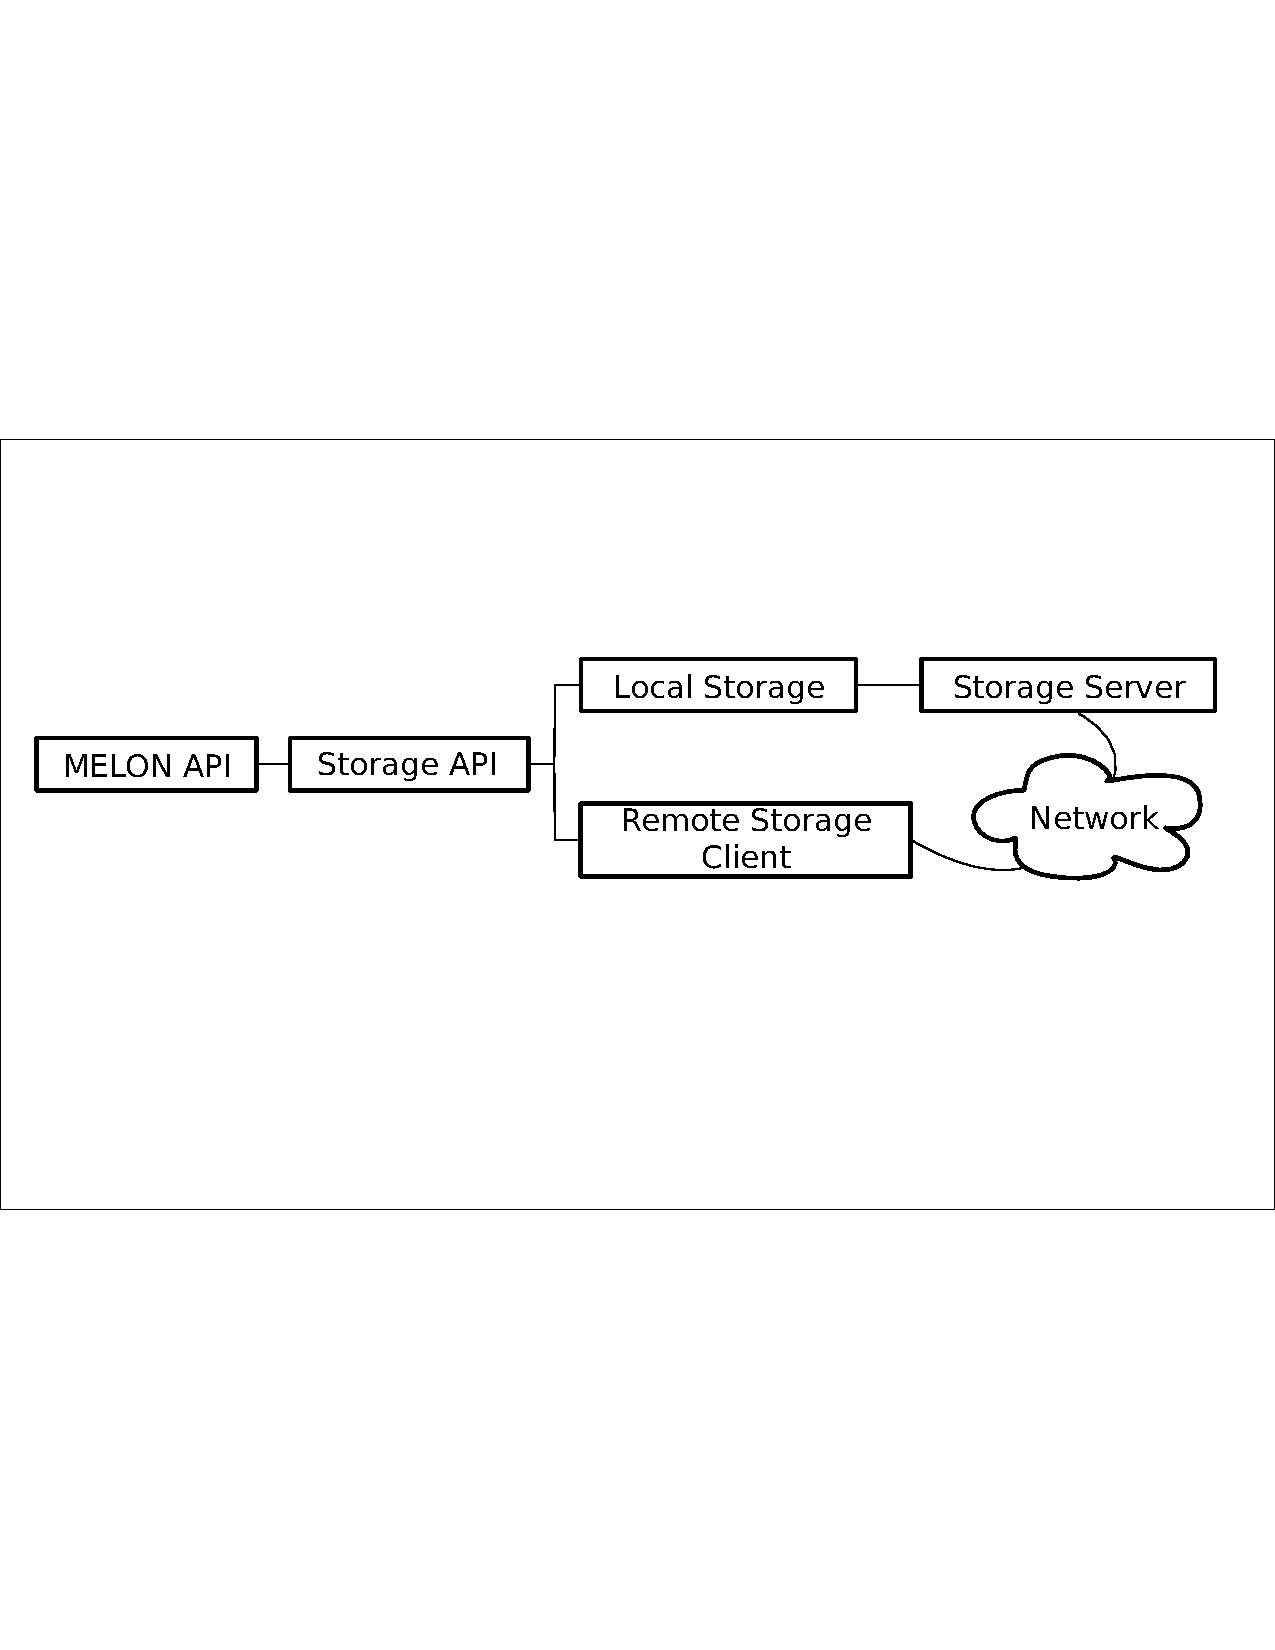
\includegraphics[scale = .50, clip, trim = 10px 280px 10px 250px]{figures/paradigm_arch.pdf}
\caption{Paradigm Architecture}
\label{fig:architecture}
\end{figure}

We developed a prototype implementation to validate our design and obtain empirical performance data. The architecture illustrated in Figure \ref{fig:architecture} is split into five parts. The Paradigm API is the only interface exposed to the application. The Paradigm API interacts with the distributed message storage through the Storage API, which provides the same interface for both local and remote storage. The Storage Server proves a network interface to a local storage space and accepts connections made through the Remote Storage stub.

Local storage is implemented simply as two vectors, one for write/read messages and the other for store/take messages. For atomic updates, the write/read vector uses a readers/writer lock to allow multiple read operations to access the vector in parallel, but locks the vector for write operations. The store/take vector does not permit parallel operations, since both store and take modify the store. The two vectors may be accessed or modified in parallel with each other.

Network communication is handled using the $\emptyset$MQ library.

\subsubsection{Tracking Read Messages}

    When a messages is stored, it is given a unique identifier [\textit{P}, \textit{M}], where \textit{P} is a globally unique integer identifier for the storing process, and \textit{M} is an integer identifier for the stored message. Each process maintains an integer ID which is incremented for each store. Messages stored from the same process with consecutive store operations will have consecutive \textit{M} values and share the same \textit{P} value.

    In order to prevent read from returning a message more than once in the same process, each process maintains a sparse bit set for each process from which a message has been read. The identifier [\textit{P}, \textit{M}] is condensed into a single unique integer \textit{Q} using the ``elegant pairing function''\cite{szudzikelegant} shown in equation \ref{eq:elegantpairing}. Since the values of \textit{Q} will be consecutive for all consecutive values of $M < P$, it is helpful to set \textit{P} to be higher than the number of expected messages. The value \textit{Q} is then stored in a sparse bit set with a hash table using integer keys and bit field values.

 \begin{equation}
   f(M,P) = \left\{
     \begin{array}{lr}
       M^{2} + M + P & : M \geq P \\
       P^{2} + M & : M < P
     \end{array}
   \right.
   \label{eq:elegantpairing}
\end{equation}

Table \ref{fig:bitset} shows an example of how the information would be stored. In this case, one byte has been used for each bit field and is displayed in binary. The index \textit{i} in the sparse bit set indicates the range stored in the bit set. If \textit{w} is the number of bits for each bit set, then each bit field can store up to \textit{w} values of \textit{n}, where $w \times i \leq n < w \times (i + 1)$. A message with ID \textit{n} will be stored in index $n \div w$ by setting the bit at $n \bmod w$ in the bit field to \texttt{1}.

If the index value is of size \textit{l} bits and the bit field contains \textit{w} bits, then the cost for storing a single value is $l + w$. For storing a set of consecutive values of length \textit{m}, the cost is $\lfloor m \times l \div w\rfloor + m$ bits. In other words, the total cost is one bit per message, plus the cost of one index per \textit{w} messages.

\begin{table}
\centering
\caption{Sparse bit set example}
\begin{tabular}{|c|c|} \hline
Index & Bit Field \\ \hline
0 & 01100001 \\ \hline
4 & 00010000 \\ \hline
15 & 10100100 \\ \hline
\end{tabular}
\label{fig:bitset}
\end{table}

Consecutive messages (from any starting value) are the best-case scenario for sparse bitsets. In the worst case, the message IDs differ by at least \textit{w}, causing each message to incur a $l + w$ cost for storage and a total cost of $m \times (l + w)$ bits.

Determining if a message [\textit{P}, \textit{M}] is in the set is accomplished by first computing \textit{Q}. If there is no key at index $Q \div w$, the message has not been read. Otherwise, retrieve the bit field \textit{b} at index $M \div w$. If $b \wedge 2^{M \bmod w} \neq 0$ then the message has been read, otherwise the message is unread.
    
\subsubsection{Retrieving Unread Messages}

When performing a \textbf{read} or \textbf{read\_all} operation, the proposed paradigm must only return messages which have not previously been returned by a \textbf{read} or \textbf{read\_all} to the requesting process. Since every process has its own set of of messages which it has read, the requesting process sends this set of read messages to the requestee.

A \textbf{read} request contains a message template and a set of messages which have already been read. The receiving process will match the message template against the messages in its local storage, excluding messages which are in the set of read messages. If a matching unread message is found, the process will send the message to the requestor. If multiple matching unread messages are found, the process will send the message with the lowest message ID. If no matching messages are found, the process returns an empty response.

Similarly, \textbf{read\_all} requests also include the message template and the set of read messages. A process receiving a \textbf{read\_all} request will match the message template against messages in the local storage, excluding messages in the set of read messages. The process will then return all matching unread messages to the requestor. If no matching unread messages are found, the process returns an empty set.

\section{Comparison to Existing Paradigms}

The proposed paradigm provides advantages over existing paradigms when used to develop applications in a MANET environment. This section compares the proposed paradigm to publish/subscribe, remote procedure calls (RPC), and tuple spaces: three paradigms often used in applications and middleware for MANETs.

\subsection{Message Persistence}

In the unreliable MANET environment, disconnections frequently occur during the exchange of messages. Since disconnections can be prolonged, the networking layers will assume the connection is entirely lost and cease attempts at retransmission.

    Publish/subscribe allows message publication without any consideration for the state of the subscribers. Publish/subscribe itself does not specify how “missed” publications should be handled. A publish/subscribe system can utilize “brokers” which manage subscriptions and facilitate delivery of publications. Brokers can then serve as message buffers and provide more reliable message delivery in the face of disconnections. In distributed publish/subscribe systems, however, the brokers must be self-organizing. For MANETs, the overhead and complexity of managing an overlay network of brokers is exacerbated by the transience of nodes. It is common, then, for distributed publish/subscribe systems to not provide any message persistence. If a subscriber is not available at the time of publication, the message will not be received by that subscriber.

    Since RPC requires a connection for any communication, disconnections typically cause RPC to block a process entirely until a remote node hosting an appropriate method is available. Messages themselves only exist briefly during the RPC transaction. Messages cannot be sent if a synchronous connection cannot be made to a remote host.
    In tuple spaces and the proposed paradigm, message persistence is inherent in the paradigms. In both paradigms, exchange of messages is achieved by storing the messages in a shared storage space, then the recipients retrieve the message from storage. Any amount of time may elapse between the storage of a message and its retrieval. This flexibility allows the communication scheme to work well even in the face of prolonged disconnections and is the reason we have chosen it for the proposed paradigm.
    
\subsection{Flexible Communication}

    A general purpose communication paradigm for MANET applications should have the flexibility to support both unicast and multicast communication.

    Publications in publish/subscribe are inherently multicast, since any number of nodes can subscribe. Unicast communication is much less comfortable in publish/subscribe, as it involves negotiating which topics should be used to identify which nodes. Publish/subscribe also does not provide any mechanism for ensuring or even acknowledging message delivery to any given subscriber, especially since publishers and subscribers are intended to be unaware of each other.

Since RPC mimics local method calls, it is natural that RPC is best suited for unicast communication, in which the message is the argument to the method and the return value is the response from the remote host. Assuming multicast RPC functions in the same manner, then a multicast RPC invocation would expect multiple return values, one from each remote host. In a MANET, it is likely not every remote host would reliably return a response, further complicating the semantics. A typical RPC invocation would block waiting for a response, but it is not practical to wait for all responses to a multicast RPC invocation, when some responses may never be received. The use of futures or asynchronous callbacks can improve the situation, but causes semantics to differ even more from unicast RPC.

    Tuple spaces are naturally multicast, since any number of nodes may read a given tuple. Unicast communication can be achieved by using a field in the tuple as the recipient’s address. The recipient then performs in operations on tuples with their address in order to receive the tuples.

    The proposed paradigm divides communications into three types: messages which can be received by any single recipient, messages which can be received by a specific single recipient, and messages which can be received by any number of recipients. Messages sent with a store operation can only be consumed by a single take operation. Directed messages are also sent with store, but can only be consumed with a take performed by the intended recipient. write stores messages which may be read by any number of recipients and can never be removed by a take. The proposed paradigm also provides the ability to receive multiple messages at once with \textbf{take\_all} and \textbf{read\_all} operations.    
    
\subsubsection{Private Communication}

    Networked applications commonly require private, unicast communication. For example: SMS services, direct messaging in social networks, or communication of sensitive data. For our purposes, private communication is the exchange of messages between two parties which cannot be disrupted or eavesdropped upon by a third party from within the context of the paradigm itself. In other words, concerns such as encrypting data or sniffing network traffic would be outside the paradigm context.

    RPC by default is unicast and there is no method in the paradigm for eavesdropping or disrupting RPC between two nodes. However, RPC has a different complication: remote hosts are generally identified by their exposed methods and there is no mechanism for attaching identity to the hosts. RPC will connect to any remote method with the expected API. So while private communication is the default in RPC, there is an addressing issue which makes it complicated to communicate with the desired recipient.

Communication in publish/subscribe is inherently public and multicast. Any subscriber can subscribe to any set of publications, making it simple to eavesdrop on communications. Bidirectional communication is also difficult in publish/subscribe, since there is no information attached to a publication indicating the identity of the publisher. This is by design, but it complicates situations in which two hosts need to converse.

In tuple spaces, tuples are public and available to any recipient. Not only can any node read any communications without detection, any node can also disrupt communications by removing tuples intended for a specific recipient.

The proposed paradigm provides two access control mechanisms for messages. First, messages are explicitly either available for any recipient to remove or limited to read-only operations. Read-only messages are useful in scenarios where information is intended to be widely available and removal of the information would be considered disruptive to the application. Second, if messages are directed to a specific recipient, then the paradigm implementation is responsible for disallowing any other nodes from reading or removing the given message. This allows simple private unicast communication between nodes.

\subsection{Multiple Read Problem}

The multiple read problem \cite{mrdp} is specific to tuple spaces: in a situation where the tuple space contains many tuples of interest, how do multiple readers read all the relevant tuples? In tuple spaces, the non-destructive rd operation returns a copy of a matching tuple, but it may return the same tuple any number of times. One solution is to use a single tuple as a mutex, lock the tuple space, remove all matching tuples with in, then replace them in the tuple space. However, this ruins any concurrency the tuple space would have had with multiple readers.

Another solution is to provide a bulk rd operation to return all matching tuples. However, once a “snapshot” of the tuple space has been taken with a bulk rd, new matching tuples may be introduced. A second bulk rd would return both the old (already seen) tuples and the new tuples.

The proposed paradigm avoids this issue by only returning messages unread by the current process. Assuming a static set of stored messages, repeated read operations in the same process would eventually return each matching message exactly once. The proposed paradigm also provides the read\_all operation for reading messages in bulk. Unlike the tuple space version, read\_all also only returns unread messages. This allows applications to easily read all existing matching messages, after which read\_all will only return messages newly added to the storage.

\section{Experimental Results}

\subsection{Setup}

In order to judge the performance of the proposed paradigm, we used applications written in the using prototype implementation and evaluated them using the EXata network emulator. Using an emulator allowed us to run real applications but also have precisely repeatable environments and scenarios.

Two scenarios were used for our experiments. In the first, nodes are placed in static positions which force multihop routes. In the second, nodes move using random waypoint at approximately walking speeds.

In both scenarios, 802.11b used blah blah...

The experiment coordination application described in the next section was used to run the applications and gather results.

\subsubsection{Coordinator}

\begin{figure}
\centering
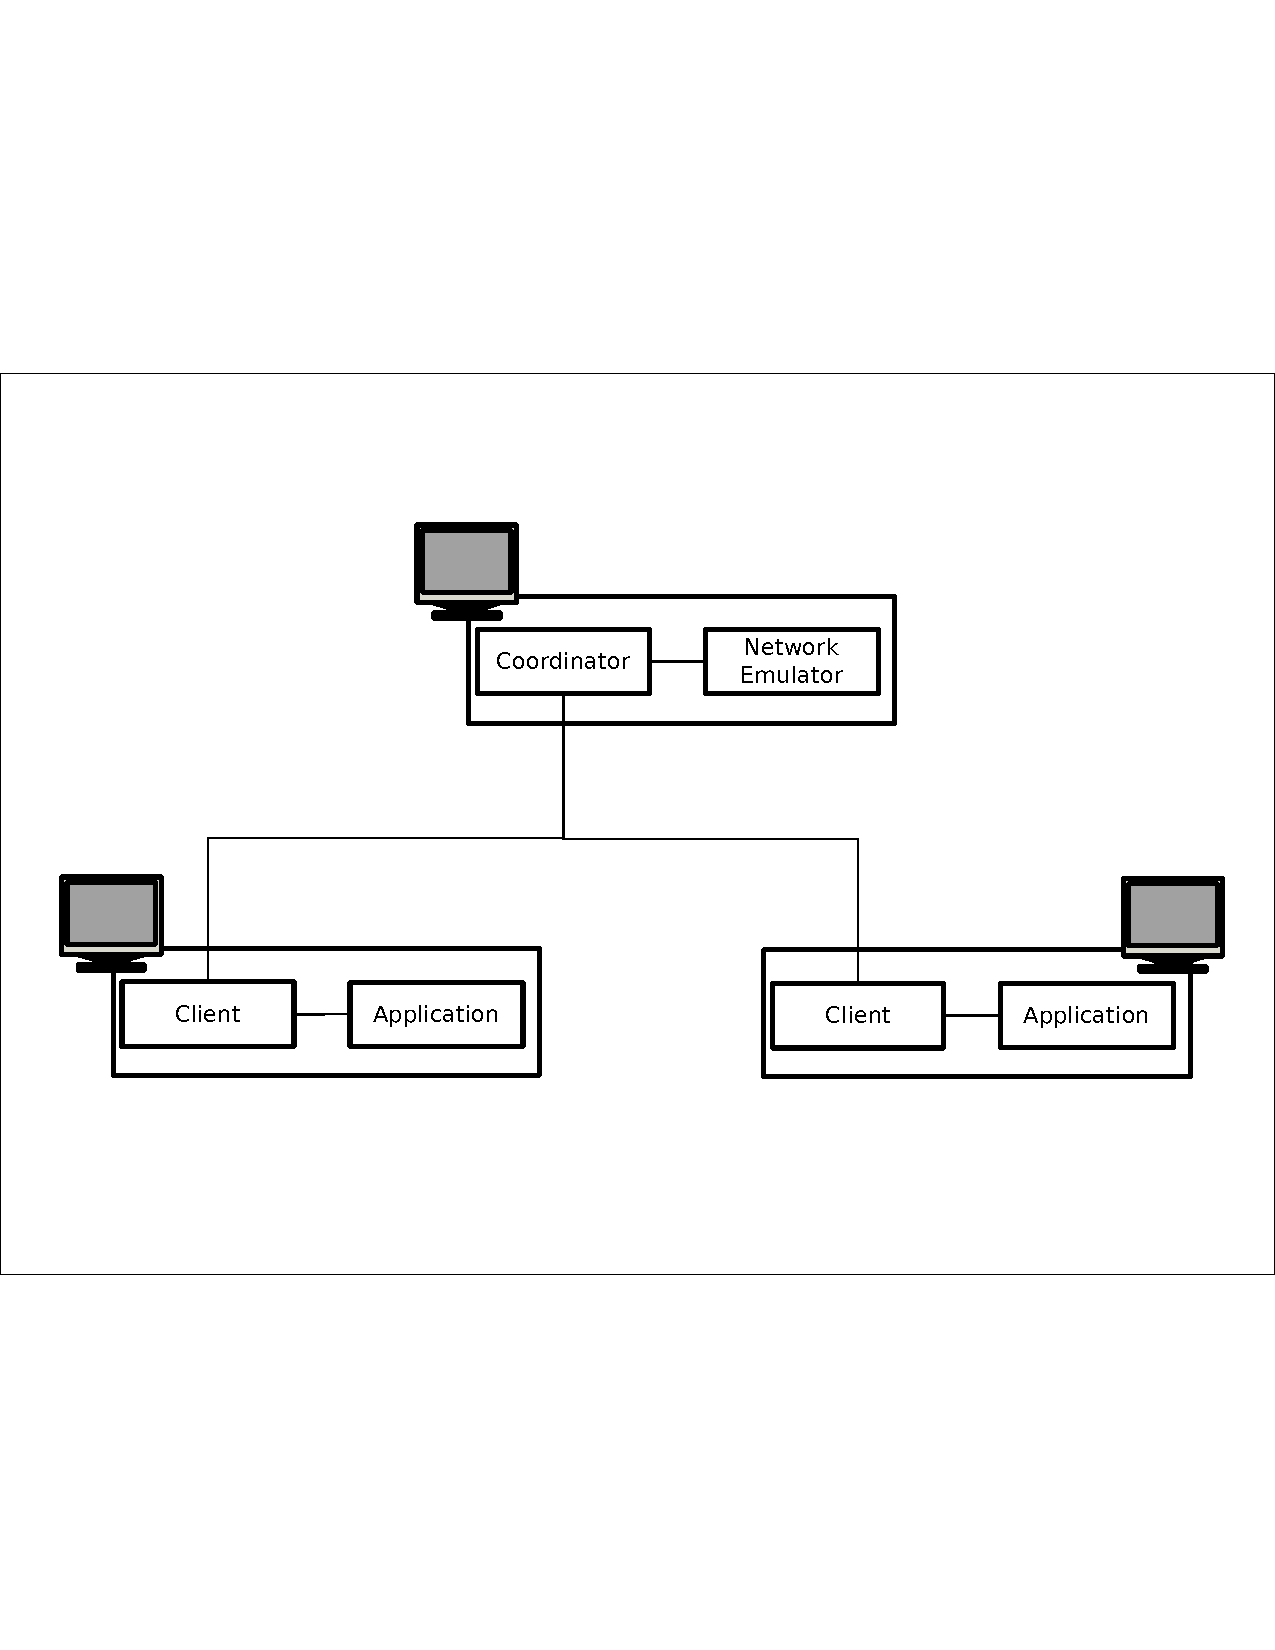
\includegraphics[scale = .50, clip, trim = 10px 240px 10px 250px]{figures/experiment_arch.pdf}
\caption{Coordinator Architecture}
\label{fig:architecture}
\end{figure}

To ease the process of repeatedly setting up experiments, we developed a framework written with the proposed paradigm which is responsible for coordinating experiments. The application handles running real applications on multiple hosts, executing the network emulator, and gathering resulting output into a single location.

The architecture of the framework is illustrated in Figure [?]. For simplicity, the coordinator resides on the same host as the network emulator. The coordinator sends out commands to clients which reside on each host. The clients are responsible for executing programs on their local host and sending resulting output to the central coordinator.

Figure[?] shows the steps the coordinator, clients, and applications use to conduct an experiment. The coordinator first writes a job containing the command to execute and any relevant options. Each client reads the job, starts the command, then stores a confirmation once the application has started and is ready to begin. When the coordinator has taken a confirmation from each host, it starts the network emulator. Then it writes a “go” message. Upon reading the go message, each client signals the application to begin.

As the application runs, the client gathers output and stores it. When the application finishes, it signals that it is done and then awaits a kill signal from the client. The client also stores a “done” signal. When the coordinator has taken a “done” message from each client, it collects the results and then sends a “kill” message. The clients then kill the applications and the process is ready to start again.

\subsection{Message Overhead}

A cost of interest for any communication paradigm is the message size overhead added for sending and receiving messages.

\subsection{Operation Speed}

To establish a baseline for performance, we measured the time for the \textbf{write}, \textbf{read}, \textbf{store}, and \textbf{take} operations directly on a local message storage and compared the results to the LighTS local tuple space implementation used by LIME.

\subsection{Message Latency}

Figures [?] and [?] show the time between the request for a message and the receipt of a matching message in both static and mobile scenarios. One host writes out 1000 messages with a 1kb payload and the other hosts read messages one at a time.

\subsection{Message Throughput}

Throughput was measured in terms of messages delivered per second. As in the other experiments, 1000 messages with a 1kb payload are output by one host, while the other hosts read the messages individually.

Since our implementation of the paradigm can easily handle concurrent reads from five hosts, the high latency seen in the experiments is the result of the wireless network.

\section{Related Work}


\section{Conclusions}


\bibliographystyle{unsrt}
\bibliography{refs}

\end{document}
